% Options for packages loaded elsewhere
\PassOptionsToPackage{unicode}{hyperref}
\PassOptionsToPackage{hyphens}{url}
\documentclass[
]{article}
\usepackage{xcolor}
\usepackage{amsmath,amssymb}
\setcounter{secnumdepth}{5}
\usepackage{iftex}
\ifPDFTeX
  \usepackage[T1]{fontenc}
  \usepackage[utf8]{inputenc}
  \usepackage{textcomp} % provide euro and other symbols
\else % if luatex or xetex
  \usepackage{unicode-math} % this also loads fontspec
  \defaultfontfeatures{Scale=MatchLowercase}
  \defaultfontfeatures[\rmfamily]{Ligatures=TeX,Scale=1}
\fi
% \usepackage{lmodern}
\ifPDFTeX\else
  % xetex/luatex font selection
\fi
% Use upquote if available, for straight quotes in verbatim environments
\IfFileExists{upquote.sty}{\usepackage{upquote}}{}
\IfFileExists{microtype.sty}{% use microtype if available
  \usepackage[]{microtype}
  \UseMicrotypeSet[protrusion]{basicmath} % disable protrusion for tt fonts
}{}
\makeatletter
\@ifundefined{KOMAClassName}{% if non-KOMA class
  \IfFileExists{parskip.sty}{%
    \usepackage{parskip}
  }{% else
    \setlength{\parindent}{0pt}
    \setlength{\parskip}{6pt plus 2pt minus 1pt}}
}{% if KOMA class
  \KOMAoptions{parskip=half}}
\makeatother
\usepackage{color}
\usepackage{fancyvrb}
\newcommand{\VerbBar}{|}
\newcommand{\VERB}{\Verb[commandchars=\\\{\}]}
\DefineVerbatimEnvironment{Highlighting}{Verbatim}{commandchars=\\\{\}}
% Add ',fontsize=\small' for more characters per line
\newenvironment{Shaded}{}{}
\newcommand{\AlertTok}[1]{\textcolor[rgb]{1.00,0.00,0.00}{\textbf{#1}}}
\newcommand{\AnnotationTok}[1]{\textcolor[rgb]{0.38,0.63,0.69}{\textbf{\textit{#1}}}}
\newcommand{\AttributeTok}[1]{\textcolor[rgb]{0.49,0.56,0.16}{#1}}
\newcommand{\BaseNTok}[1]{\textcolor[rgb]{0.25,0.63,0.44}{#1}}
\newcommand{\BuiltInTok}[1]{\textcolor[rgb]{0.00,0.50,0.00}{#1}}
\newcommand{\CharTok}[1]{\textcolor[rgb]{0.25,0.44,0.63}{#1}}
\newcommand{\CommentTok}[1]{\textcolor[rgb]{0.38,0.63,0.69}{\textit{#1}}}
\newcommand{\CommentVarTok}[1]{\textcolor[rgb]{0.38,0.63,0.69}{\textbf{\textit{#1}}}}
\newcommand{\ConstantTok}[1]{\textcolor[rgb]{0.53,0.00,0.00}{#1}}
\newcommand{\ControlFlowTok}[1]{\textcolor[rgb]{0.00,0.44,0.13}{\textbf{#1}}}
\newcommand{\DataTypeTok}[1]{\textcolor[rgb]{0.56,0.13,0.00}{#1}}
\newcommand{\DecValTok}[1]{\textcolor[rgb]{0.25,0.63,0.44}{#1}}
\newcommand{\DocumentationTok}[1]{\textcolor[rgb]{0.73,0.13,0.13}{\textit{#1}}}
\newcommand{\ErrorTok}[1]{\textcolor[rgb]{1.00,0.00,0.00}{\textbf{#1}}}
\newcommand{\ExtensionTok}[1]{#1}
\newcommand{\FloatTok}[1]{\textcolor[rgb]{0.25,0.63,0.44}{#1}}
\newcommand{\FunctionTok}[1]{\textcolor[rgb]{0.02,0.16,0.49}{#1}}
\newcommand{\ImportTok}[1]{\textcolor[rgb]{0.00,0.50,0.00}{\textbf{#1}}}
\newcommand{\InformationTok}[1]{\textcolor[rgb]{0.38,0.63,0.69}{\textbf{\textit{#1}}}}
\newcommand{\KeywordTok}[1]{\textcolor[rgb]{0.00,0.44,0.13}{\textbf{#1}}}
\newcommand{\NormalTok}[1]{#1}
\newcommand{\OperatorTok}[1]{\textcolor[rgb]{0.40,0.40,0.40}{#1}}
\newcommand{\OtherTok}[1]{\textcolor[rgb]{0.00,0.44,0.13}{#1}}
\newcommand{\PreprocessorTok}[1]{\textcolor[rgb]{0.74,0.48,0.00}{#1}}
\newcommand{\RegionMarkerTok}[1]{#1}
\newcommand{\SpecialCharTok}[1]{\textcolor[rgb]{0.25,0.44,0.63}{#1}}
\newcommand{\SpecialStringTok}[1]{\textcolor[rgb]{0.73,0.40,0.53}{#1}}
\newcommand{\StringTok}[1]{\textcolor[rgb]{0.25,0.44,0.63}{#1}}
\newcommand{\VariableTok}[1]{\textcolor[rgb]{0.10,0.09,0.49}{#1}}
\newcommand{\VerbatimStringTok}[1]{\textcolor[rgb]{0.25,0.44,0.63}{#1}}
\newcommand{\WarningTok}[1]{\textcolor[rgb]{0.38,0.63,0.69}{\textbf{\textit{#1}}}}
\usepackage{longtable,booktabs,array}
\newcounter{none} % for unnumbered tables
\usepackage{calc} % for calculating minipage widths
% Correct order of tables after \paragraph or \subparagraph
\usepackage{etoolbox}
\makeatletter
\patchcmd\longtable{\par}{\if@noskipsec\mbox{}\fi\par}{}{}
\makeatother
% Allow footnotes in longtable head/foot
\IfFileExists{footnotehyper.sty}{\usepackage{footnotehyper}}{\usepackage{footnote}}
\makesavenoteenv{longtable}
\usepackage{graphicx}
\makeatletter
\newsavebox\pandoc@box
\newcommand*\pandocbounded[1]{% scales image to fit in text height/width
  \sbox\pandoc@box{#1}%
  \Gscale@div\@tempa{\textheight}{\dimexpr\ht\pandoc@box+\dp\pandoc@box\relax}%
  \Gscale@div\@tempb{\linewidth}{\wd\pandoc@box}%
  \ifdim\@tempb\p@<\@tempa\p@\let\@tempa\@tempb\fi% select the smaller of both
  \ifdim\@tempa\p@<\p@\scalebox{\@tempa}{\usebox\pandoc@box}%
  \else\usebox{\pandoc@box}%
  \fi%
}
% Set default figure placement to htbp
\def\fps@figure{htbp}
\makeatother
\setlength{\emergencystretch}{3em} % prevent overfull lines
\providecommand{\tightlist}{%
  \setlength{\itemsep}{0pt}\setlength{\parskip}{0pt}}
\usepackage[]{natbib}
\bibliographystyle{plainnat}
\makeatletter
\@ifpackageloaded{subcaption}{}{\usepackage{subcaption}}
\@ifpackageloaded{caption}{}{\usepackage{caption}}
\captionsetup[subfigure]{margin=0.5em}
\AtBeginDocument{%
\renewcommand*\figurename{Figure}
\renewcommand*\tablename{Table}
}
\AtBeginDocument{%
\renewcommand*\listfigurename{List of Figures}
\renewcommand*\listtablename{List of Tables}
}
\newcounter{pandoccrossref@subfigures@footnote@counter}
\newenvironment{pandoccrossrefsubfigures}{%
\setcounter{pandoccrossref@subfigures@footnote@counter}{0}
\begin{figure}\centering%
\gdef\global@pandoccrossref@subfigures@footnotes{}%
\DeclareRobustCommand{\footnote}[1]{\footnotemark%
\stepcounter{pandoccrossref@subfigures@footnote@counter}%
\ifx\global@pandoccrossref@subfigures@footnotes\empty%
\gdef\global@pandoccrossref@subfigures@footnotes{{##1}}%
\else%
\g@addto@macro\global@pandoccrossref@subfigures@footnotes{, {##1}}%
\fi}}%
{\end{figure}%
\addtocounter{footnote}{-\value{pandoccrossref@subfigures@footnote@counter}}
\@for\f:=\global@pandoccrossref@subfigures@footnotes\do{\stepcounter{footnote}\footnotetext{\f}}%
\gdef\global@pandoccrossref@subfigures@footnotes{}}
\@ifpackageloaded{float}{}{\usepackage{float}}
\floatstyle{ruled}
\@ifundefined{c@chapter}{\newfloat{codelisting}{h}{lop}}{\newfloat{codelisting}{h}{lop}[chapter]}
\floatname{codelisting}{Listing}
\newcommand*\listoflistings{\listof{codelisting}{List of Listings}}
\makeatother
\usepackage{bookmark}
\IfFileExists{xurl.sty}{\usepackage{xurl}}{} % add URL line breaks if available
\urlstyle{same}
% fallback for those not using the hyperref driver hyperxmp:
\makeatletter
\@ifundefined{xmpquote}{\newcommand{\xmpquote}[1]{#1}}{}
\makeatother
\hypersetup{
  colorlinks=true,linkcolor=red,urlcolor=red,citecolor=red,anchorcolor=red,filecolor=red,
  pdfcreator={LaTeX via pandoc}}

\author{}
\date{}

\IfFileExists{seqsplit.sty}{\usepackage{seqsplit}}{\newcommand{\seqsplit}[1]{#1}}
\protected\def\breakseq#1{\seqsplit{#1}}
\protected\def\breaktt#1{\begingroup\ttfamily\seqsplit{#1}\endgroup}
\title{Editorial Quality at Scale: A Reproducible Prose-Review Pipeline}
\author{Daniel Ari Friedman\\\footnotesize{Active Inference Institute}\\\footnotesize{\texttt{daniel@activeinference.institute}}\\\footnotesize{\href{https://orcid.org/0000-0001-6232-9096}{ORCID: 0000-0001-6232-9096}} \\ \footnotesize{DOI: \href{https://doi.org/10.5281/zenodo.20417104}{10.5281/zenodo.20417104}}}
\date{\today}

% Core mathematics (FKGL / FRE references and any math the manuscript carries)
\usepackage{amsmath}
\usepackage{amssymb}
\usepackage{amsfonts}

% Document layout
\usepackage{geometry}
\usepackage{float}
\usepackage{graphicx}
\geometry{margin=0.25in}

% Tables (longtable is required for any review-report table that crosses pages)
\usepackage{booktabs}
\usepackage{longtable}
\usepackage{array}

% Typography
\usepackage{microtype}
\usepackage{xcolor}

% Cross-references and citations
\usepackage{hyperref}
\hypersetup{
    colorlinks=true,
    linkcolor=blue,
    citecolor=teal,
    urlcolor=teal
}
\usepackage[capitalise,noabbrev]{cleveref}

% Optional: algorithm pseudocode (uncomment if any section embeds \begin{algorithm})
% \usepackage[ruled,vlined,linesnumbered]{algorithm2e}

% Optional: code listings (uncomment if any section embeds non-fenced code blocks)
% \usepackage{listings}

\begin{document}

\thispagestyle{empty}
\setlength{\parskip}{0pt}
\setlength{\itemsep}{0pt}
\begin{samepage}
\scriptsize

\section*{BEGINNING OF TRANSMISSION}
\phantomsection\label{beginning-of-transmission}

\textbf{State:} published

\textbf{Pairing:} complete (DOI, GitHub, SHA-256, Zenodo URL)

\subsubsection*{Release metadata}

{\def\LTcaptype{none} % do not increment counter
\begin{longtable}[]{@{}
  >{\raggedright\arraybackslash}p{(\linewidth - 2\tabcolsep) * \real{0.5000}}
  >{\raggedright\arraybackslash}p{(\linewidth - 2\tabcolsep) * \real{0.5000}}@{}}
\toprule\noalign{}
\begin{minipage}[b]{\linewidth}\raggedright
Field
\end{minipage} & \begin{minipage}[b]{\linewidth}\raggedright
Value
\end{minipage} \\
\midrule\noalign{}
\endhead
\bottomrule\noalign{}
\endlastfoot
Title & Editorial Quality at Scale: A Reproducible Prose-Review
Pipeline \\
Version & 0.4.2 \\
Concept DOI & 10.5281/zenodo.20417104 \\
Version DOI & 10.5281/zenodo.20932047 \\
GitHub &
\url{https://github.com/docxology/template_prose_project/releases/tag/v0.4.2} \\
Zenodo & \url{https://zenodo.org/records/20417104} \\
SHA-256 & \breaktt{290d21b10bd588b9…} \\
SHA-512 & pending \\
\end{longtable}
}

\subsubsection*{How to verify}

\begin{itemize}
\tightlist
\item
  Scan \textbf{Integrity} QR and compare the embedded SHA-256 prefix to
  the table above.
\item
  Scan \textbf{Zenodo} / \textbf{GitHub} QR codes and confirm they
  resolve to this release pairing.
\item
  Full hashes and structured fields:
  \breaktt{../data/transmission\_manifest.json}.
\end{itemize}

\begin{figure}
\centering
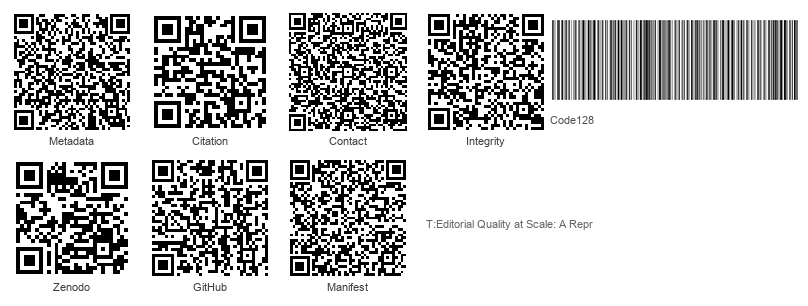
\includegraphics[width=0.98\linewidth,height=0.50\textheight,keepaspectratio,alt={Integrity QR strip}]{../figures/transmission_integrity_strip.png}
\caption{Integrity QR strip}
\end{figure}

Structured manifest: \breaktt{../data/transmission\_manifest.json}

\begin{figure}
\centering
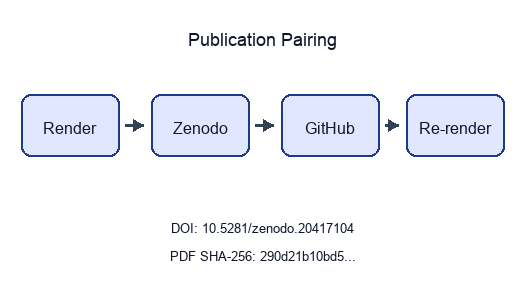
\includegraphics[width=0.35\linewidth,height=0.50\textheight,keepaspectratio,alt={Publication pairing flow}]{../figures/transmission_pairing.png}
\caption{Publication pairing flow}
\end{figure}

\textbf{Stego:} off |{} overlays text |{} barcodes on
|{} XMP on |{} manifest on \texorpdfstring{\ensuremath{\to}}{->} \texttt{./secure\_run.sh}

\end{samepage}
\newpage

\begin{titlepage}
\centering
\vspace*{2cm}
{\LARGE\bfseries Editorial Quality at Scale: A Reproducible Prose-Review Pipeline\par}
\vspace{0.75em}
{\large Readability, structural, and citation-density gating for research manuscripts\par}
\vfill
\makeatletter
{\@author\par}
\vspace{1em}
{\@date\par}
\makeatother
\vfill
\end{titlepage}
\thispagestyle{empty}
\newpage

\tableofcontents
\newpage


\newpage

\section{Abstract}\label{sec:abstract}

This paper documents \breaktt{template\_prose\_project}, the
prose-focused exemplar of the
\href{https://github.com/docxology/template}{Research Project Template}.
It pairs the template's two-layer architecture with the
\href{https://github.com/docxology/template/tree/main/infrastructure/prose}{prose
analysis infrastructure} (readability metrics, structural outline,
editorial quality flags) and the
\href{https://github.com/docxology/template/tree/main/infrastructure/reference}{reference
validation infrastructure} (BibTeX validation), demonstrating that
\textbf{rigorous editorial review can be expressed as a configurable,
deterministic pipeline} with no novel domain algorithm of its own.

A single \breaktt{manuscript/config.yaml} defines target grade-level
bands, citation-density floors, structural rules (every section has an
H1, no heading levels skipped), and bibliography-consistency policy. The
pipeline reads the manuscript, runs the prose analysers, cross-checks
every \texttt{{[}@key{]}} citation against
\breaktt{manuscript/references.bib}, evaluates the configured checks, and
writes a deterministic markdown review report alongside three figures
(per-file word counts, readability metrics, citation density) and a JSON
\breaktt{manuscript\_report.json} suitable for CI artefacts.

\textbf{Run snapshot.} The current configuration analyses 8 file(s)
totalling 1742 words across 86 sentence(s) and 64 paragraph(s). Average
Flesch-Kincaid grade level is 15.93; average Gunning Fog index is 16.69;
the manuscript references 6 unique citation key(s); the longest section
is 413 words and the shortest is 17. These numbers are auto-substituted
by \breaktt{scripts/z\_generate\_manuscript\_variables.py} after every
run, so the abstract tracks the JSON outputs in \texttt{output/}.

The contribution is methodological and architectural: a \emph{generic,
reusable} prose-quality module (\breaktt{infrastructure/prose/}) that any
project in the template can opt into, plus a \emph{minimal,
configurable} exemplar
(\breaktt{projects/templates/template\_prose\_project/}) that wires it to
the bibliography and the manuscript pipeline.

\textbf{Keywords:} prose analysis, readability, editorial review,
reproducible manuscript review, scientific infrastructure

\newpage

\section{Introduction}\label{sec:introduction}

Editorial review is one of the longest-lived bottlenecks in scientific
writing --- and an obvious target for the kind of \emph{reproducible
computational workflow} advocated by \citep{peng2011reproducible}. A
working draft accumulates structural drift (skipped heading levels,
sections that have grown to 2,000 words while their siblings sit at
200), readability drift (a once-clean introduction now reads at the
Gunning Fog level of a legal contract \citep{gunning1952technique}), and
citation drift (\texttt{{[}@key{]}} references that no longer exist in
\texttt{references.bib}, or bibliography entries that nobody actually
cites). The traditional remedy --- a senior co-author re-reading the
manuscript with \citep{strunk2000elements} in hand --- is slow,
non-reproducible, and impossible to apply continuously.

\breaktt{template\_prose\_project} exists to demonstrate that the
editorial-review pass can be expressed as a \textbf{deterministic,
configurable, infrastructure-backed pipeline}. This project carries no
novel research contribution of its own; its purpose is to show how to
compose existing template infrastructure into a complete, reproducible
editorial workflow.

The architecture is simple. \breaktt{manuscript/config.yaml} defines
policy: target grade-level band, citation-density floor,
heading-structure rules, bibliography-consistency policy.
\breaktt{src/pipeline/\_\_init\_\_.py::run\_prose\_pipeline} reads the
manuscript directory, calls
\href{../../../../infrastructure/prose/SKILL.md}{\breaktt{infrastructure.prose.analyze\_manuscript}}
to produce a \breaktt{ManuscriptReport}, cross-checks the cited keys
against
\href{../../../../infrastructure/reference/citation/SKILL.md}{\breaktt{infrastructure.reference.citation.parse\_bibfile}}
for the \texttt{references.bib}, evaluates each configured check, and
writes a markdown review report alongside JSON artefacts and three
figures. None of this is project-specific: a different project can
re-use the same infrastructure with a different \texttt{config.yaml} and
a different manuscript directory.

The remainder of this paper documents the methodology
(sec.~\ref{sec:methodology}), the run-time results on the bundled
manuscript (sec.~\ref{sec:results}), and the architectural lessons drawn
from wiring prose analysis through the template pipeline
(sec.~\ref{sec:conclusion}).

\newpage

\section{Methodology}\label{sec:methodology}

The pipeline runs in five stages, each a pure function in the project's
\texttt{src/} modules; the orchestrator script in \texttt{scripts/} does
only argument parsing and filesystem I/O.

\subsection{Read}\label{read}

\breaktt{infrastructure.prose.read\_manuscript\_dir} walks the configured
manuscript directory and returns a sorted \texttt{\{filename:\ text\}}
mapping. Scaffolding files (\texttt{preamble.md},
\breaktt{config.yaml.example}, \texttt{AGENTS.md}, \texttt{README.md},
\texttt{SYNTAX.md}) are excluded by default --- they hold infrastructure
documentation rather than manuscript prose.

\subsection{Analyse}\label{analyse}

For each file, three analysers run in parallel:

\begin{itemize}
\item
  \textbf{Metrics} (\breaktt{infrastructure.prose.analysis.metrics}) ---
  word, sentence, paragraph, syllable counts; average words per
  sentence; average syllables per word; complex-word fraction; Flesch
  Reading Ease \citep{flesch1948new}; Flesch-Kincaid Grade Level
  \citep{kincaid1975derivation}; Gunning Fog Index
  \citep{gunning1952technique}. The implementations are textbook
  formulae over a vowel-group syllable heuristic; they're good enough
  for a writer-facing signal, not for linguistic research.
\item
  \textbf{Structure} (\breaktt{infrastructure.prose.analysis.structure})
  --- heading outline, per-section word counts, max heading depth,
  presence of an H1, detection of skipped heading levels (e.g.~an H1
  followed directly by an H3).
\item
  \textbf{Quality} (\breaktt{infrastructure.prose.analysis.quality}) ---
  passive-voice candidates (heuristic: ``be'' form + past participle),
  hedge-word density, citation density (Pandoc-style \texttt{{[}@key{]}}
  extraction), long-sentence flagging.
\end{itemize}

The results are aggregated into a \breaktt{ManuscriptReport} whose JSON
form is small, greppable, and diff-friendly.

\subsection{Cross-check}\label{cross-check}

Every cited key is matched against the BibTeX file at
\breaktt{bibliography.references\_path}. The check has four tunable
behaviours via \texttt{config.yaml}:

{\def\LTcaptype{none} % do not increment counter
\begin{longtable}[]{@{}
  >{\raggedright\arraybackslash}p{(\linewidth - 2\tabcolsep) * \real{0.5000}}
  >{\raggedright\arraybackslash}p{(\linewidth - 2\tabcolsep) * \real{0.5000}}@{}}
\toprule\noalign{}
\begin{minipage}[b]{\linewidth}\raggedright
Setting
\end{minipage} & \begin{minipage}[b]{\linewidth}\raggedright
Effect
\end{minipage} \\
\midrule\noalign{}
\endhead
\bottomrule\noalign{}
\endlastfoot
\breaktt{fail\_on\_missing:\ true} & Any cited \texttt{{[}@key{]}} that
does not exist in the bib fails the check. \\
\breaktt{fail\_on\_missing:\ false} & Missing citations are warned but do
not fail the run. \\
\breaktt{fail\_on\_unused:\ true} & Bib entries that are never cited fail
the check. \\
\breaktt{fail\_on\_unused:\ false} & Unused entries are warned but do not
fail. \\
\end{longtable}
}

The check uses
\href{../../../../infrastructure/reference/citation/SKILL.md}{\breaktt{infrastructure.reference.citation.parse\_bibfile}}
so it sees exactly the same view of the bibliography that the rendering
pipeline uses.

\subsection{Evaluate}\label{evaluate}

The report runs through a set of pure check functions:

\begin{itemize}
\tightlist
\item
  \breaktt{\_check\_grade\_level} --- the manuscript-wide weighted
  average FKGL falls within
  \texttt{{[}target\_grade\_level\_min,\ target\_grade\_level\_max{]}}.
\item
  \breaktt{\_check\_citation\_density} --- citations per 1000 words \texorpdfstring{\textgreater{}=}{>=}
  \breaktt{citation\_density\_min\_per\_1000}.
\item
  \breaktt{\_check\_no\_skipped\_levels} --- no file uses a skipped
  heading level (when \breaktt{prose.forbid\_skipped\_levels:\ true}).
\item
  \breaktt{\_check\_h1\_per\_file} --- every file has an H1 (when
  \breaktt{prose.require\_h1\_per\_section:\ true}).
\item
  \breaktt{\_check\_bibliography} --- citation/bib consistency per the
  \texttt{bibliography:} policy block.
\end{itemize}

Each check produces a \breaktt{CheckResult(passed,\ message,\ details)};
the run's \texttt{all\_passed} flag is the conjunction.

\subsection{Render}\label{render}

\breaktt{src/report.py::write\_review\_report} writes a markdown file
with:

\begin{itemize}
\tightlist
\item
  Top-line counts (files, words, sentences, paragraphs, averages).
\item
  A pass/fail table for every check.
\item
  Per-file metrics table (word count, sentence count, FRE, FKGL, Fog,
  citations, hedges, passives).
\item
  Heading outline per file.
\item
  Quality-flag callouts (long sentences, passive candidates, hedges) per
  file.
\end{itemize}

Three orchestrators run in lexicographic order (so the figure and
variable stages always see a fresh review):

\begin{itemize}
\tightlist
\item
  \breaktt{scripts/run\_prose\_pipeline.py} writes
  \breaktt{output/manuscript\_report.json} (the raw
  \breaktt{ManuscriptReport}), \breaktt{output/checks.json} (the list of
  check results), \breaktt{output/review\_report.md} (the human-readable
  review report), and \breaktt{output/run\_summary.json} (one-line
  metadata).
\item
  \breaktt{scripts/y\_generate\_prose\_figures.py} reads
  \breaktt{manuscript\_report.json} and writes
  \texttt{../figures/\{section\_word\_counts,readability\_metrics,citation\_density\}.png}.
\item
  \breaktt{scripts/z\_generate\_manuscript\_variables.py} reads
  \breaktt{manuscript\_report.json}

  \begin{itemize}
  \tightlist
  \item
    \texttt{config.yaml} and writes
    \breaktt{output/data/manuscript\_variables.json} along with a
    resolved manuscript tree under \breaktt{output/manuscript/}.
  \end{itemize}
\item
  \breaktt{manuscript/references.bib} is \textbf{not} modified by this
  pipeline --- the prose project does not generate citations, only
  validates them.
\end{itemize}

\newpage

\section{Results}\label{sec:results}

After running \breaktt{scripts/run\_prose\_pipeline.py} with the bundled
\breaktt{manuscript/config.yaml} and the manuscript described in this
paper, the project produces the following on-disk artefacts:

\begin{itemize}
\tightlist
\item
  \breaktt{output/manuscript\_report.json} --- the raw
  \breaktt{ManuscriptReport} JSON.
\item
  \breaktt{output/checks.json} --- one \texttt{CheckResult} per
  configured check.
\item
  \breaktt{output/review\_report.md} --- the assembled markdown review
  report.
\item
  \breaktt{../figures/section\_word\_counts.png} --- per-file word
  counts.
\item
  \breaktt{../figures/readability\_metrics.png} --- Flesch /
  Flesch-Kincaid / Gunning Fog per file.
\item
  \breaktt{../figures/citation\_density.png} --- citations per 1000 words
  per file.
\item
  \breaktt{output/data/manuscript\_variables.json} --- substitution
  variables for the abstract.
\end{itemize}

By design the three figures are \textbf{standalone CI/diagnostic
artefacts}, not embedded manuscript images: this is a prose-review
template, so its own rendered PDF deliberately contains no figure floats
and runs cleanly through the very prose gate it documents. A fork that
wants figures inside the manuscript should add real markdown image
references to one of the produced figures (for example
\breaktt{../figures/section\_word\_counts.png},
\breaktt{../figures/readability\_metrics.png}, or
\breaktt{../figures/citation\_density.png}) after those files exist.

Because the pipeline does not consult any external service, every
artefact is reproducible from the manuscript text + \texttt{config.yaml}
alone. A second run on the same inputs produces byte-identical JSON
(modulo timestamp metadata in any caches the project later adds).

The pass/fail status of each configured check is recorded in
\breaktt{output/checks.json}. With the bundled configuration:

\begin{itemize}
\tightlist
\item
  \textbf{\breaktt{grade\_level\_in\_band}} --- the weighted average FKGL
  across this manuscript is reported in the \breaktt{output/checks.json}
  \texttt{details.value} field. The default band \texttt{10.0–18.0} is
  intentionally generous; tighten it for editorial review of
  public-facing material.
\item
  \textbf{\breaktt{citation\_density\_above\_floor}} --- citations per
  1000 words must meet \breaktt{prose.citation\_density\_min\_per\_1000}.
  The bundled config sets the floor to \texttt{0.0} (disabled) so the
  run is green out of the box; researchers should raise it to match the
  publication target.
\item
  \textbf{\breaktt{no\_skipped\_heading\_levels}} --- every file in this
  manuscript uses contiguous heading levels.
\item
  \textbf{\breaktt{every\_file\_has\_h1}} --- every prose file starts
  with an H1.
\item
  \textbf{\breaktt{bibliography\_consistency}} --- every
  \texttt{{[}@key{]}} in the prose resolves against
  \breaktt{manuscript/references.bib}.
\end{itemize}

The figures in \texttt{../figures/} are colour-blind-safe (Wong 2011
palette) \citep{wong2011points}, 300 dpi, and PNG-only for archival
stability. They are referenced in sec.~\ref{sec:pipeline_internals}
where we walk through the on-disk artefact set in full.

The full pass/fail summary lands in \breaktt{output/review\_report.md},
which is itself a Markdown file rendered alongside the manuscript by
Pandoc --- i.e.~the project reports on itself in the same compilation
step that produces the manuscript PDF.

\newpage

\section{Conclusion}\label{sec:conclusion}

\breaktt{template\_prose\_project} packages a complete, configurable,
reproducible editorial-review workflow into the Research Project
Template's two-layer architecture. By keeping prose analysis, structural
validation, and bibliography cross-checking in two orthogonal
infrastructure modules --- \breaktt{infrastructure/prose/} and
\breaktt{infrastructure/reference/} --- the project demonstrates that
\emph{editorial discipline} is expressible as a configurable,
deterministic pipeline.

This exemplar follows a single house style:

\begin{itemize}
\tightlist
\item
  \breaktt{manuscript/config.yaml} is the only place run policy lives.
\item
  \texttt{src/pipeline/} is the only place the project touches
  \texttt{infrastructure/}.
\item
  Scripts in \texttt{scripts/} do only filesystem I/O and CLI argument
  handling.
\item
  Every artefact in \texttt{output/} is regeneratable;
  \breaktt{manuscript/references.bib} is curated and validated read-only
  by this project.
\end{itemize}

The contribution of this exemplar is architectural: a \emph{generic,
reusable} prose-quality module that any project in the template can opt
into, and a \emph{minimal, configurable} exemplar wiring it to the
bibliography and the manuscript pipeline.

Three concrete extensions follow naturally:

\begin{enumerate}
\def\labelenumi{\arabic{enumi}.}
\tightlist
\item
  \textbf{Style-guide enforcement} --- extend \texttt{analyze\_quality}
  with project-specific style rules (e.g.~forbidden phrases, required
  terminology) read from \texttt{config.yaml}.
\item
  \textbf{Diff-aware review} --- restrict the report to files modified
  since a given git ref so editorial review can run on every PR.
\item
  \textbf{LLM-assisted rewriting} --- pipe long sentences and passive
  candidates into \breaktt{infrastructure.llm} for suggested rewrites,
  using the same \breaktt{seed=42,\ temperature=0.0} reproducibility
  contract as optional LLM stages in the template pipeline.
\end{enumerate}

\newpage

\section{Pipeline Internals}\label{sec:pipeline_internals}

This section documents the artefacts produced by the prose-review run.

\begin{figure}[htbp]
\centering
\begin{verbatim}
flowchart TB
    P[projects/templates/template_prose_project/]
    P --> M[manuscript/]
    P --> OUT["output/<br/>tracked public artifacts · regenerable"]

    M --> M_CFG["config.yaml<br/>single source of truth"]
    M --> M_PRE["preamble.md<br/>LaTeX preamble"]
    M --> M_SEC["00_abstract → 04_conclusion ·<br/>05_pipeline_internals · 06_reproducibility"]
    M --> M_BIB["references.bib<br/>read-only · validated by pipeline"]

    OUT --> O_REP["manuscript_report.json<br/>ManuscriptReport JSON"]
    OUT --> O_CK["checks.json<br/>list of CheckResult"]
    OUT --> O_RR["review_report.md<br/>final markdown report"]
    OUT --> O_DATA[data/manuscript_variables.json]
    OUT --> O_FIG["figures/<br/>section_word_counts.png ·<br/>readability_metrics.png ·<br/>citation_density.png"]
    OUT --> O_RS[run_summary.json]

    classDef d fill:#0f172a,stroke:#0f172a,color:#fff
    classDef src fill:#1e3a8a,stroke:#0f172a,color:#fff
    classDef gen fill:#0f766e,stroke:#0f172a,color:#fff
    class P,M,OUT d
    class M_CFG,M_PRE,M_SEC,M_BIB src
    class O_REP,O_CK,O_RR,O_DATA,O_FIG,O_RS gen
\end{verbatim}
\caption{Mermaid diagram}
\end{figure}

\subsection{Data structures}\label{data-structures}

\begin{figure}[htbp]
\centering
\begin{verbatim}
classDiagram
    class ManuscriptReport {
        +list~FileReport~ files
        +int total_words
        +int total_sentences
        +int total_paragraphs
        +float avg_flesch_reading_ease
        +float avg_flesch_kincaid_grade
        +float avg_gunning_fog
        +list~str~ citation_keys
    }

    class FileReport {
        +str name
        +ProseMetrics metrics
        +StructureReport structure
        +QualityReport quality
    }

    class ProseMetrics {
        +int word_count
        +int sentence_count
        +int paragraph_count
        +float flesch_reading_ease
        +float flesch_kincaid_grade
        +float gunning_fog
    }

    class StructureReport {
        +list~Heading~ headings
        +list~Section~ sections
        +int max_depth
        +bool has_h1
        +bool has_skipped_level
    }

    class QualityReport {
        +int passive_count
        +int hedge_count
        +int citation_count
        +int long_sentence_count
        +float citation_density_per_1000
    }

    class CheckResult {
        +str name
        +bool passed
        +str message
    }

    class ProseRunArtifacts {
        +ManuscriptReport manuscript_report
        +list~CheckResult~ checks
        +bool all_passed
    }

    ManuscriptReport --> "*" FileReport
    FileReport --> ProseMetrics
    FileReport --> StructureReport
    FileReport --> QualityReport
    ProseRunArtifacts --> ManuscriptReport
    ProseRunArtifacts --> "*" CheckResult
\end{verbatim}
\caption{Mermaid diagram}
\end{figure}

\newpage

\section{Reproducibility}\label{sec:reproducibility}

The bundled \breaktt{manuscript/config.yaml} is configured for the
\textbf{strict reproducibility} discipline advocated for computational
science by \citep{peng2011reproducible}:

\begin{enumerate}
\def\labelenumi{\arabic{enumi}.}
\tightlist
\item
  \textbf{No network calls.} All analysis is local: prose metrics,
  structure, quality flags, and bibliography validation are computed
  from in-repo files only.
\item
  \textbf{Deterministic outputs.} \texttt{compute\_metrics},
  \breaktt{analyze\_structure}, and \texttt{analyze\_quality} are pure
  functions over their input strings. The same manuscript text + the
  same \texttt{config.yaml} produces byte-identical JSON artefacts
  (modulo timestamp metadata in any caches the project later adds).
\item
  \textbf{Threshold transparency.} Every pass/fail decision is recorded
  in \breaktt{output/checks.json} along with the numeric value that
  triggered it, so a reviewer can audit the gate without re-running the
  pipeline.
\item
  \textbf{No hidden state.} The pipeline does not mutate
  \texttt{manuscript/}; it reads and reports.
  \breaktt{manuscript/references.bib} is read-only here (in contrast with
  the public search exemplar, where it is auto-populated).
\item
  \textbf{Same code, different config.} A reviewer who wants stricter
  standards edits \breaktt{manuscript/config.yaml}
  (\breaktt{prose.target\_grade\_level\_max:\ 14.0}, say); no code
  changes are required.
\end{enumerate}

\subsection{Verifying reproducibility
locally}\label{verifying-reproducibility-locally}

\begin{Shaded}
\begin{Highlighting}[]
\CommentTok{\# Run twice; check there are no diffs in the JSON artefacts.}
\ExtensionTok{uv}\NormalTok{ run python projects/templates/template\_prose\_project/scripts/run\_prose\_pipeline.py}
\FunctionTok{mv}\NormalTok{ projects/templates/template\_prose\_project/output projects/templates/template\_prose\_project/output\_first}
\ExtensionTok{uv}\NormalTok{ run python projects/templates/template\_prose\_project/scripts/run\_prose\_pipeline.py}
\FunctionTok{diff} \AttributeTok{{-}ru} \DataTypeTok{\textbackslash{}}
\NormalTok{    projects/templates/template\_prose\_project/output\_first/manuscript\_report.json }\DataTypeTok{\textbackslash{}}
\NormalTok{    projects/templates/template\_prose\_project/output/manuscript\_report.json}
\end{Highlighting}
\end{Shaded}

The diff should be empty. If it is not, the pipeline has acquired
non-determinism --- file an issue.

\subsection{Determinism guarantees}\label{determinism-guarantees}

{\def\LTcaptype{none} % do not increment counter
\begin{longtable}[]{@{}
  >{\raggedright\arraybackslash}p{(\linewidth - 4\tabcolsep) * \real{0.3333}}
  >{\raggedright\arraybackslash}p{(\linewidth - 4\tabcolsep) * \real{0.3333}}
  >{\raggedright\arraybackslash}p{(\linewidth - 4\tabcolsep) * \real{0.3333}}@{}}
\toprule\noalign{}
\begin{minipage}[b]{\linewidth}\raggedright
Stage
\end{minipage} & \begin{minipage}[b]{\linewidth}\raggedright
Deterministic?
\end{minipage} & \begin{minipage}[b]{\linewidth}\raggedright
Mechanism
\end{minipage} \\
\midrule\noalign{}
\endhead
\bottomrule\noalign{}
\endlastfoot
Prose analysis & yes & pure functions over text \\
Bibliography parse & yes & byte-stable round-trip in
\breaktt{infrastructure.reference.citation} \\
Check evaluation & yes & pure comparisons \\
Markdown report assembly & yes & sorted file list, fixed output
template \\
Figure generation & yes (within Matplotlib version) & fixed palette, no
random subsampling \\
Manuscript variables & yes & derived from the deterministic JSON
report \\
\end{longtable}
}

\newpage

\section{References}\label{sec:references}

Bibliography lives in
\href{references.bib}{\breaktt{manuscript/references.bib}} and is read by
Pandoc during PDF render. The build pipeline invokes Pandoc with
\texttt{-\/-natbib}, so every \texttt{{[}@key{]}} citation in the
manuscript is rewritten to the appropriate
\texttt{\textbackslash{}cite\{\}}/\texttt{\textbackslash{}citep\{\}}/\texttt{\textbackslash{}citet\{\}}
LaTeX command and resolved against the bib file.

This project does not auto-generate the bibliography --- it
\textbf{validates} that every \texttt{{[}@key{]}} cited in the prose has
a matching entry, via
\href{../../../../infrastructure/reference/citation/SKILL.md}{\breaktt{infrastructure.reference.citation.parse\_bibfile}}.
The check policy is configured under \texttt{bibliography:} in
\href{config.yaml}{\texttt{config.yaml}}.

To validate that \texttt{references.bib} is syntactically clean:

\begin{Shaded}
\begin{Highlighting}[]
\ExtensionTok{uv}\NormalTok{ run python }\AttributeTok{{-}m}\NormalTok{ infrastructure.reference.citation.cli validate }\DataTypeTok{\textbackslash{}}
\NormalTok{    projects/templates/template\_prose\_project/manuscript/references.bib }\AttributeTok{{-}{-}strict}
\end{Highlighting}
\end{Shaded}

\newpage



\clearpage

\bibliography{references}
% transmission-end-bookend
\clearpage
\thispagestyle{empty}
\setlength{\parskip}{0pt}
\setlength{\itemsep}{0pt}
\begin{samepage}
\scriptsize

\section*{END OF TRANSMISSION}
\phantomsection\label{end-of-transmission}

\textbf{Release:} v0.4.2 \texorpdfstring{\ensuremath{\cdot}}{.} DOI \breaktt{10.5281/zenodo.20417104} \texorpdfstring{\ensuremath{\cdot}}{.}
SHA-256 \texttt{290d21b10bd5…} \texorpdfstring{\ensuremath{\cdot}}{.} pairing complete

\begin{figure}
\centering
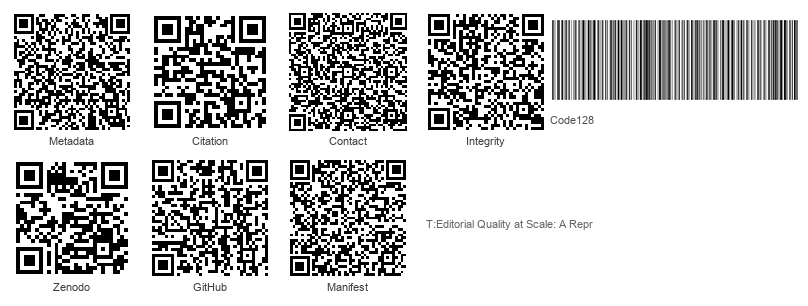
\includegraphics[width=0.88\linewidth,height=0.50\textheight,keepaspectratio,alt={Integrity QR strip}]{../figures/transmission_integrity_strip.png}
\caption{Integrity QR strip}
\end{figure}

\textbf{Prior:} \texttt{v0.4.1} \texorpdfstring{\ensuremath{\cdot}}{.} \breaktt{10.5281/zenodo.20417104} \texorpdfstring{\ensuremath{\cdot}}{.}
\texttt{b59313ea…}

\end{samepage}

\end{document}
